\documentclass[11pt]{article}
%\documentclass{ametsoc}
\usepackage{natbib}
\usepackage{graphicx}
\usepackage{wrapfig}
\usepackage{rotating}
\usepackage{amsmath}
\usepackage{graphicx}
\usepackage{multicol}
\usepackage{natbib}
\usepackage{wrapfig}
\usepackage{hyperref}
\usepackage{tabularx}
\usepackage{setspace}
\usepackage{comment}
\usepackage{bibentry} 
\usepackage{color}

\usepackage[compact]{titlesec}  
\titlespacing{\section}{0pt}{0pt}{0pt}
\titlespacing{\subsection}{0pt}{0pt}{-5pt}
\titlespacing{\subsubsection}{0pt}{0pt}{-5pt}

\oddsidemargin 0cm
\evensidemargin 0cm

\parindent 0cm
\parskip 0.5cm

\usepackage{fancyhdr}
\pagestyle{plain}
\fancyfoot[C]{Page \thepage}

\usepackage[margin=1in]{geometry}

%\title{\textbf{Modeling the Effect of Regional Climate Change in the Western USA: An Assessment of Mountain Snowpack}}

%\author{Dr. Paul Ullrich (PI)}
%\date{ }
   
\begin{document}

\bibliographystyle{ametsoc2014}  
\nobibliography{MountainSnowpack}

%\maketitle

%\tableofcontents
%\newpage

\section{Project Description}
\subsection{Background and Summary}
The next century will see unprecedented changes to the climate system. The most well understood trends (such as increasing global surface temperature) are of a broad global nature and do not necessarily reflect changes on regional scales, which are key for planning on all levels. For this reason, developing a scientific understanding of changing regional climate is an unmet challenge that must be addressed. Regional climate change is particularly important to California, one of the most environmentally and agriculturally diverse regions in the world. With around two-thirds of California's developed water supply originating from the Sierra Nevada, there is growing concern that climate change will directly alter the tendencies of this natural reservoir of water.  The primary source of freshwater from this region comes in the form of winter snowpack, providing one-third of California's available water.  As global temperatures rise, snowpack is expected to decline dramatically and melt earlier in the season.  These two factors will assuredly stem late summer water flow which is integral to maintaining agricultural, environmental, and municipal water needs.  Modeling snowpack accurately requires the need for high model resolution to represent large-scale and convective snow systems, topography (with resulting orographic forcing and snow line representation), and the overall fractal nature of snow cover extent and depth. To address our understanding of these features, this proposal advances the use of a next generation modeling tool to better understand regional climate change and its effect on snowpack in California and the broader western USA.
\\\\
The \textbf{central objective} of this work is to better understand how climate change will affect water resources in the western USA, specifically water associated with mountain snowpack.  We postulate that although global climate change will not lead to a significant change in total precipitation throughout the western states, this region (and specifically California) will see shifts in precipitation storage, due to changes in precipitatio timing, spatial distribution and type, with a steady decline in winter snowpack, especially in lower elevation basins.  The magnitude and extent of these changes remains a key question.  In order to address this, our work will utilize a multitude of climate model, observational, and reanalysis datasets to provide a comprehensive assessment of how water resources are changing.  A unique strength and theme of this proposal is the use of \textbf{variable-resolution global modeling systems (VRGCMs)}, which have the capacity to achieve high spatial resolution over a limited-area region.
\\\\
The key \textbf{scientific questions} that will be addressed by this proposal are as follows:

\begin{itemize}
\item[(Q1)] How accurately do VRGCMs represent the timing of snowfall?  How accurately do VRGCMs represent the spatial distribution, depth, total Snow Water Equivalent (SWE) and melt rate of snowpack throughout the western US?  How sensitive are these indicators to the the underlying grid resolution?

\item[(Q2)] Quantitatively, how will west coast mountain snowpack (both total snowpack and on the scale of specific basins) be affected by future climate?  How will interannual variability be affected?

\item[(Q3)] How will the spatial distribution of mountain snowpack change in response to anticipated global changes in general circulation?

\item[(Q4)] How will atmospheric rivers respond to anticipated changes in circulation, and how will these changes affect the spatial distribution and total accumulation of mountain snowpack?
\end{itemize}

\noindent The \textbf{central hypotheses} for this proposal are:
\begin{itemize}
\item[(H1)] VRGCMs are a statistically informative and cost-effective method to characterize snowfall and snowpack trends within the Sierra Nevada (and western USA) compared to conventional standard resolution general circulation model runs used by the Intergovernmental Panel on Climate Change (IPCC) and standard regional climate model simulations
\item[(H2)] Sierra Nevada snowpack trends will see a significant decline, in the coming century, with a shift towards more rain and less snow, earlier peak accumulation and melt onset, and more dramatic impacts felt on lower elevation basins.
\item[(H3)] Atmospheric rivers and, consequently, precipitation will experience a poleward shift in response to changes in the general circulation.
\end{itemize}

\noindent To address these hypotheses, the following \textbf{research plan} will be pursued:
\begin{itemize}
\item[(T1)] Validate and evaluate the capability of VRGCMs \textbf{Community Earth System Model (CESM)} and the \textbf{Model for Prediction Across Scales (MPAS)} to represent mountain snowpack at different spatial resolutions, with different physical parameterizations and under different tunings.  For comparison, we will also assess the widely-used Weather Research and Forecasting (WRF) regional model, and uniform resolution CESM model simulations.
\item[(T2)] Analyze the capability of the Community Land Model (CLM) to represent snowpack at SNOTEL station locations using meteorology forced from VRGCMs.
\item[(T3)] Use CESM and MPAS to assess changes in mountain snowpack in response to changes in atmospheric greenhouse gas concentrations prescribed by the suite of Relative Concentration Pathways (RCPs).
\item[(T4)] Detect and characterize atmospheric river events in variable-resolution simulations in terms of total over-land precipitation, total accumulated snowfall and position of landfall.
%\item Provide a scientifically robust assessment of both historical and future 21st century (Present-2100) changes that may affect California and the broader western USA's hydrologic future, with specific interest in mountain snowpack. 
\item[(T5)] Develop regional climate data and statistics for follow-up applications including policymaking, water management, and regional climate change research.
%\item Generate new tools that spur easier assessment of the reliability and scientific value of variable resolution modeling systems. 
\end{itemize}

\noindent This research fits well within the objectives of the Climate and Large-Scale Dynamics program, with its focus on processes that govern climate, the causes of climate variability and change, methods to predict climate variations, extended weather and climate predictability, and the use of climate models to diagnose and simulate climate and its variations and change.

\subsection{Broader Impacts and Intellectual Merit}

\subsubsection{Broader Impacts}

This research will have broad ranging benefits across atmospheric, hydrologic, computer science, and western USA decision making communities.  VRGCMs will allow us to transcend long held scientific paradigms through the use of a global climate model (CESM) with model grid resolutions that water managers and policy makers may find relevant to make more informed regional management and policy decisions.  The western USA is a unique hydroclimate regime in which snowpack provides the vast majority of freshwater resources (especially during summer months), has shown steady decline over the last half century, depends upon global teleconnections, and faces major uncertainties in its climate change resiliency.  Our hope is that VRGCMs will lead to a new hybrid form of global/regional climate modeling, more realistic modeled outcomes, and assessment of how CESM performs at resolved scales (<50km) currently not used in standard practice.  This technique could have broad ranging impacts across the climate science field, but must first be scientifically tested and vetted to assess its performance in comparison to historical observations, reanalysis datasets, and traditionally used climate models.  In addition, a key objective of this proposal is to make a concerted effort towards communicating and developing climate model tools and data that is more accessible and usable for agency managers and decision makers alike.

\subsubsection{Intellectual Merit}

To date, the climate modeling community has largely been forced to work within one of two scientific paradigms, global climate modeling or regional climate modeling.  Each method has their own unique benefits as well as their own major physical assumptions, computer hardware limitations and model biases.  The proposed research aims to push the boundaries of both global climate modeling and regional climate modeling through a new novel approach, Variable Resolution Global Climate Modeling (VRGCM).  This will be one of the first studies that uses the VRGCM technique to address real scientific questions and the first to use the new variable resolution capability of the Community Earth System Model (CESM) to address hydroclimatology topics within the western USA (a hydrologically sensitive and susceptible region).  Additionally, an expected outcome of our proposed research will be the development of new tools for assessing the reliability and scientific value of variable resolution modeling systems. 

\subsubsection{Strengths of the Investigation Team}

PI Ullrich has extensive first-hand experience with atmospheric model development, having developed a global shallow-water model \citep{ullrich2010high}, a regional atmospheric modeling system \citep{ullrich2012operator} and a fully 3D non-hydrostatic dynamical core \citep{ullrich2012mcore}. Further, he has worked on adaptive mesh refinement and quasi-uniform grid geometries in extensive detail \citep{collins2013nonhydrostatic}. He is heavily involved in national collaborations on climate projects, and is an organizer on a number of sessions and workshops which are related to atmospheric modeling. In addition, he is closely affiliated with ongoing climate research efforts at Lawrence Berkeley National Laboratory (LBNL) and NCAR. He is currently working on the question of extreme weather detection and attribution for extratropical cyclones and pressure blocking events leading to heat waves along with students Marielle Pinheiro and Josephine Fong. As part of a summer internship they are working jointly with the PI, Dr. Michael Wehner (LBNL) and others on the LBNL climate research team (Bill Collins, Dan Martin, Daıthı Stone, Prabhat, and others).

Dr.  Shu-Hua Chen (UC Davis) has extensive experience with using WRF for regional atmospheric modeling and so will be a valuable collaborator towards the completion of this project. She will be assisting with the use of WRF for simulating the snowpack, as well as coupling WRF to the CESM ensemble data. {\color{red}[More here]}

The PI and his collaborating team are uniquely positioned to conduct multi-model ensemble intercomparisons using a suite of cutting-edge atmospheric models and post-processing tools. This award will not only serve as a springboard for the PI's future career, but will also provide a framework for future variable resolution intercomparison studies and an improved understanding of hydroclimate effects facing California (and the broader western USA).

\subsection{Present state of knowledge}

The climate system consists of complex interactions on a variety of scales. Changes in the climate system, which occur on the timescale of decades, inherently necessitate a global approach to ensure that these scale interactions are accurately captured by models. This requirement has made it difficult to diagnose changes to regional climate which occur due to shifts in the whole Earth system. Further, restrictions on computational cost have inherently limited the finest resolution of our uniform-resolution global climate models to resolutions of around 50km, which is insufficient for resolving regional scale variability, fine-scale weather events, and topography. As stated in the National Center for Atmospheric Research (NCAR) 2009-2014 strategic plan, \textit{human-induced global climate change has been largely accepted as real, but information about temperature changes are not at a sufficiently fine scale for planning regional adaptation and mitigation} \citep{NCAR2009}. Consequently, the development of high-resolution regional climate simulations and associated uncertainty metrics is among the top NCAR short-term imperatives \citep{NCAR2009}. Recent advances in global Earth system modeling have focused on the development of variable resolution global climate models (VRGCMs) as a means for better understanding interactions between the global and regional scale and to improve climate projections over a limited area.  VRGCMs utilize a global coarse resolution grid which is refined over a specific area of interest; hence, these models often require only 10 percent of the computing power of uniform resolution models to resolve fine-scale features. These efforts are now beginning to come to fruition, and have led to Earth system models which both correctly capture regional-global interactions and reach the resolutions needed to understand regional climate change.   As part of its objective, this proposal addresses the need for additional development and testing of these models for tackling real scientific problems.

\subsubsection{Mountain Snowpack}

Regional climate change is particularly important to California, one of the most biologically and environmentally diverse regions in the world. The agricultural industry in California is responsible for roughly 50 percent of the nation’s fruit and vegetable production, and is particularly susceptible to extreme weather events and sudden changes in regional climate. Western mountain snowpack is a crucial reservoir for precipitation from California’s wet winters (providing 75 percent of freshwater supplies), and is an important mechanism for the gradual release of this water during the typically dry summer \citep{cayan1996interannual}. In particular, summer snowmelt is an incredibly important source of agricultural water \citep{dettinger1995large, mote_declining_2005, maurer2007detection}. Recent trends in water availability have projected a potentially significant loss of agricultural water associated with loss of snow melt \citep{dyer2006spatial}. In particular, the 2013-2014 snow season was one of the driest years on record in California (one-fifth of normal), with water reserves at record lows, resulting in repercussions that were felt throughout the California Central Valley agricultural communities.

Climate change directly impacts mountain snowpack via two avenues: First, warming temperatures lead to an earlier spring thaw, increasing runoff associated with spring melt and decreasing late summer water availability due to early depletion of snowpack. Second, warmer air holds more water and so leads to an increase in both large-scale and convective precipitation, although warmer temperatures also tends to favor rainfall over snowfall. Anomalous warm temperatures are particularly important in the spring at mid- to high-elevations, which would normally be below freezing throughout the winter period \citep{cayan1996interannual,stewart2009changes}. Evidence of climate change on mountain snowpack in the western US has primarily been served via empirical studies focused on April 1st measured snow depth, which has suggested there is clear evidence of a decline in snowpack throughout the western US everywhere except in the southern Sierra Nevadas \citep{mote_declining_2005}. Accumulation in this region has been attributed to an increase in the strength of the North American monsoon \citep{dyer2006spatial}. Other studies have corroborated this conclusion \citep{dettinger1995large,mote_declining_2005,knowles2006trends} and suggested that warming of the Earth's climate will lead to a continual decline in snow resources. Further, many of these studies have demonstrated that (\textit{although the trends presented here may be partially attributable to interdecadal climate variability associated with the Pacific decadal oscillation, they also appear to result from still longer-term climate shifts}) \citep{knowles2006trends}. Current trends suggest that there will be a continued decline in mountain snowpack \citep{stewart2009changes}. Regions for which the hydrological cycle is dependent on the availability of water resources originating from melting snow or ice are expected to be particularly hard hit, with potentially dramatic effects on ecology and agriculture \citep{barnett2005potential}.

In order to obtain a robust prediction of snow water availability in the next century, global atmospheric models must be used to capture the long time scales associated with the changing climate.  However, mountain snow cover exhibits fractal-like characteristics and strong topographical dependence that makes it difficult to capture at the typical resolutions of global models. Consequently, an accurate treatment of snowpack requires grid resolution which is much finer than modern global models can produce. Hence either using dynamical downscaling to a high resolution regional model, such as the Weather Research and Forecasting (WRF) model \citep{michalakes2001development}, or a global model that captures different spatial scales, such as a VRGCM, is necessary to study modeled snowpack in a global context.

\subsubsection{Observational datasets}

Observational datasets for snowpack metrics such as snow water equivalent (SWE), snow depth (SNOWDP), and snow cover (SNOWC) are inherently hard to capture in mountainous environments.  The fractal nature of snowpack deposits, quick shifts in elevation, angular differences in topography, alpine vegetation cover, cloud cover, and large footprint radius associated with satellite instrumentation pose challenges in resolving spatially continuous snowpack products \citep{brownandmote2009, rutter2009SnowMIP2}.  Additionally, many satellite products span less than a decade which inhibits analysis of climate patterns over decadal timeframes.  In-situ measurements help to get around some of the highlighted issues, yet they are inherently discontinuous.  Land surface models (LSM) have been used to abate the discontinuous nature of in situ observations, but may pose bias in the true state of the system.  Further, it has been shown that SWE and SNOWDP measurement error can be hard to quantify, but bias of around 10.5 percent has been seen \citep{ rutter2009SnowMIP2}.  Therefore, to try and address the multitudes of complications associated with snowpack metrics and assessment, a comprehensive blend of the aforementioned data types will be used to analyze the VRGCM climate simulations. 

There are several datasets that this study will use for validation purposes (Table \ref{t1}).  Each dataset varies in snowpack product availability, spatial and temporal resolution, map projection, and temporal range.  To provide more optimal comparisons, the aforementioned datasets will be standardized to monthly averaged, seasonally averaged (DJF), and climate averaged (25 year DJF) temporal resolutions during the assessment of the VRGCM simulations.  In order to accomplish this task, utilities from the NetCDF Operator (NCO), Climate Data Operator (CDO), and the NCAR Command Language (NCL) will be used \citep{schulzweida2007cdo,zender2006netcdf}.  

\begin{table*}[t]
\caption{Datasets, and associated metadata, used to analyze the accuracy of the Variable Resolution Global Climate Model (VRGCM) simulations}\label{t1}
\begin{center}
\begin{tabular*}{\textwidth}{@{\extracolsep\fill}lcccccccc}
\hline
Dataset & Snowpack  Product & Spatial  Resolution & Temporal Resolution \\
\hline
 CMC & SWE, SNOWDP & 24km & Daily\\
 DAYMET & SWE & 1km & Daily \\
 MODIS/Terra & SNOWC & 5km & Monthly \\
 SNOTEL/Snow Course & SWE, SNOWDP & 24 Stations & Daily \\
 NARR & SNOWDP, SNOWC & 32km & Daily \\
 NCEP (CFSV2) & SWE, SNOWDP, SNOWC & 35km & Daily \\
\hline
 Uniform CESM & SWE, SNOWDP, SNOWC & 28km & Daily \\
 WRF & SWE, SNOWDP, SNOWC & 27km, 9km & Daily \\
\hline
\end{tabular*}
\end{center}
\end{table*}

The Canadian Meteorological Centre (CMC) SNOWDP dataset is comprised of surface synoptic observations and meteorological aviation reports from the World Meteorological Organization’s information system.  CMC derives SWE values using the aforementioned SNOWDP measurements and look-up tables for snow density values \citep{brown2003gridded}.  The DAYMET dataset provides SWE estimations from interpolated meteorological stations.  The interpolated station data is then extrapolated, using a truncated Guassian weighting filter, to create a high resolution gridded output \citep{thornton2012daymet}.  The Moderate Resolution Imaging Spectroradiometer (MODIS) satellite dataset provides SNOWC using a snow mapping algorithm with a Normalized Difference Snow Index (NDSI) \citep{salomonson2006development}.  The NDSI is used to distinguish between snow and other features (such as cloud cover) by using visible and short wave near IR spectral bands \citep{salomonson2006development}.  The SNOwpack TELemetry (SNOTEL) in situ dataset is comprised of 24 automated observational stations spread throughout the Sierra Nevada mountain range measuring SNOWDP and SWE \citep{serreze1999characteristics}.  The areal extent of the SNOTEL stations range from 38.07$^{o}$ to 42.99$^{o}$ latitude by -120.79$^{o}$ to -119.23$^{o}$ with an average elevation of 2343.45 meters.  In addition to maintaining the SNOTEL automated station dataset, the Natural Resources Conservation Service (NRCS) also takes in situ snow course measurements of SNOWDP and SWE by trained observers at 32 permanent sites.  The measurements are taken during the first of every month in January through May along a 305 meter long transect line, usually in small meadow areas, with an average elevation of 2293.01 meters.  The North American Regional Reanalysis (NARR) dataset provides monthly averaged SNOWDP and SNOWC output variables using a high resolution atmospheric model (Eta Model) forced by a Regional Data Assimilation System (RDAS) \citep{mesinger2006north}.  The other reanalysis dataset (NCEP - CFSV2) that will be used is a recently updated (2013) version of its predecessor (2004).  The NCEP dataset provides improved two meter surface temperature, MJO, and SST forecasts while upgrading overall performance in seasonal/subseasonal forecasting results, compared to its predecessor \citep{saha2014ncep}. NCEP has also been advised for use by decision makers in the water management and agricultural fields \citep{saha2014ncep}.  Two 0.25$^{o}$ uniform resolution (spectral element and finite-volume dynamical cores) CESM datasets will be used to intercompare with the VRGCM simulations too.  These two simulations were conducted by a team at Lawrence Berkeley National Laboratories (LBNL). To provide added benefit to the proposal, we will compare the VRGCM simulations to a pair of regional climate model (RCM) simulations too.  A pair of simulations will be conducted at UC Davis using an (out of the box) version (V3.5.1) of the Weather Research and Forecasting (WRF) model, a widely used RCM.  The simulations will use a multi-resolution domain with a coarse resolution of 27km and a finer resolution domain of 9km situated over the western USA (centered on the Sierra Nevada).  Both WRF domains provide SWE, SNOWDP, and SNOWC output variables.

\subsubsection{Variable Resolution Global Climate Modeling (VRGCMs)}

The Community Earth-System Model (\citet{hurrell2013community}, CESM) is a state-of-the-art Earth modeling framework developed at NCAR, consisting of atmospheric, oceanic, land and sea ice components. This framework has been under development for nearly two decades, and has been used heavily in better understanding the effects of global climate change. The Community Atmosphere Model (CAM, the atmospheric component of CESM) is further broken into two components: the dynamical core, which solves the 3-D primitive equations of motion for the atmosphere, and the physics parameterization suite, which incorporates processes that occur on scales below the model grid scale. Because of its modular nature, CAM currently allows for switching between four dynamical cores, including the finite-volume, semi-Lagrangian, Eulerian and spectral element dynamical cores, with work underway for the inclusion of others in the near future. Of these four, only one dynamical core has variable resolution capability, namely the CAM spectral element (SE) dynamical core (CAM-SE).

The spectral element method has several important properties including parallel scalability, flexibility and accuracy, that make it a desirable choice for modeling atmospheric dynamics.  The spectral element dynamical core \citet{fournier2004spectral, taylor2010compatible} is now the default dynamical core in CAM and so is a supported platform for scientific research. Recently CAM-SE has added variable resolution support which allows for coupled climate simulations in CAM on a variable resolution atmospheric mesh. The mesh must be conformal, so each edge is shared by exactly two quadrilateral spectral elements. Two of the meshes that we will use are depicted in Figure \ref{fig:CESMVarResMeshes}, which shows smooth refinement over North America from a global resolution of 1.0$^{o}$ to a refined region with 0.25$^{o}$ (right) and 0.125$^{o}$ (left) grid spacing over the US west coast.  We have also incorporated variable resolution grids into the land surface model of CESM (CLM).  This is a new breakthrough that will unify the two meshes in both CESM components and eliminate potential grid to grid interpolation issues.  There have been recent modeling efforts using variable resolution support in CAM-SE including both short-term weather forecasting and longer-term climate forecasting, with an interest in obtaining hurricane counts in the Atlantic basin \citep{zarzycki2014using}.

\begin{figure}
  \begin{center}
  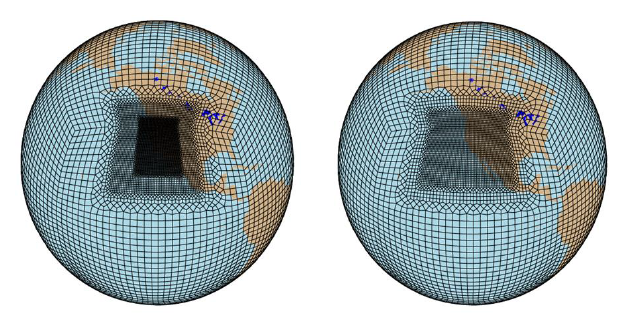
\includegraphics[width=0.75\textwidth]{14kmand28kmgrids}
  \caption{The two Variable Resolution Global Climate Model (VRGCM) grids (14km, left, and 28km, right) implemented into the Community Earth System Model (CESM) for this study.  Both grids base resolution are 1$^{o}$ cubed-sphere.  Over the western USA, a halving of resolution in each distinct domain region occurs with the inner most domain featuring a 14km resolution (left) and 28km resolution (right).} \label{fig:CESMVarResMeshes}
  \end{center}
\end{figure}

\begin{figure}
  \begin{center}
  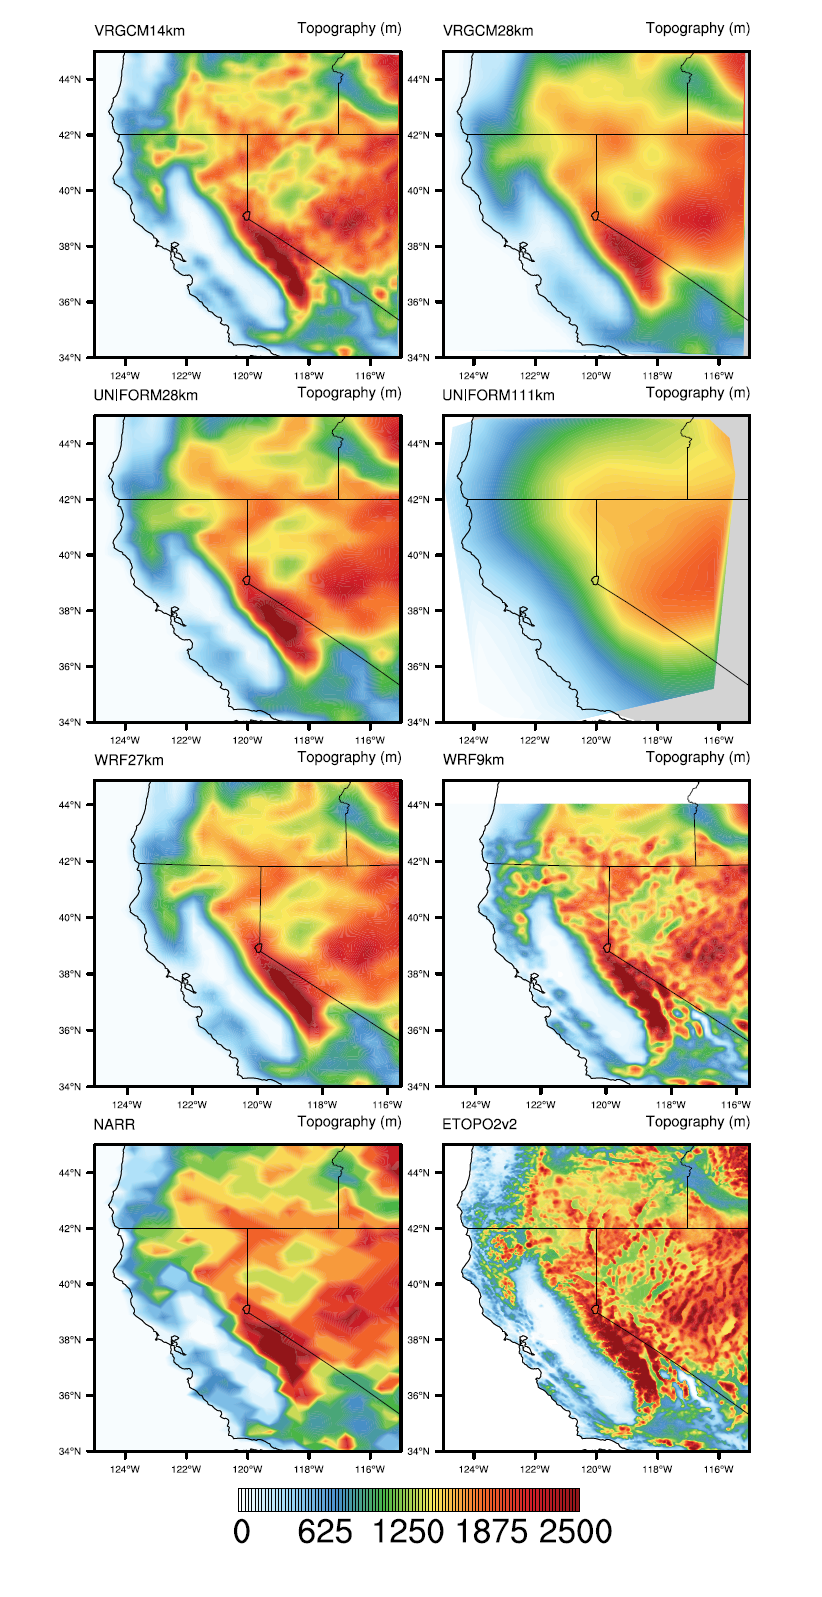
\includegraphics[width=10cm,height=25cm,keepaspectratio]{Topography}
  \caption{\label{f3}  Topography representations in the VRGCM, WRF, standard resolution CESM, and reanalysis datasets compared to a close proximity to reality (NOAA's ETOPO2v2 2km dataset) for California}
  \end{center}
\end{figure}

\begin{figure}
\begin{center}
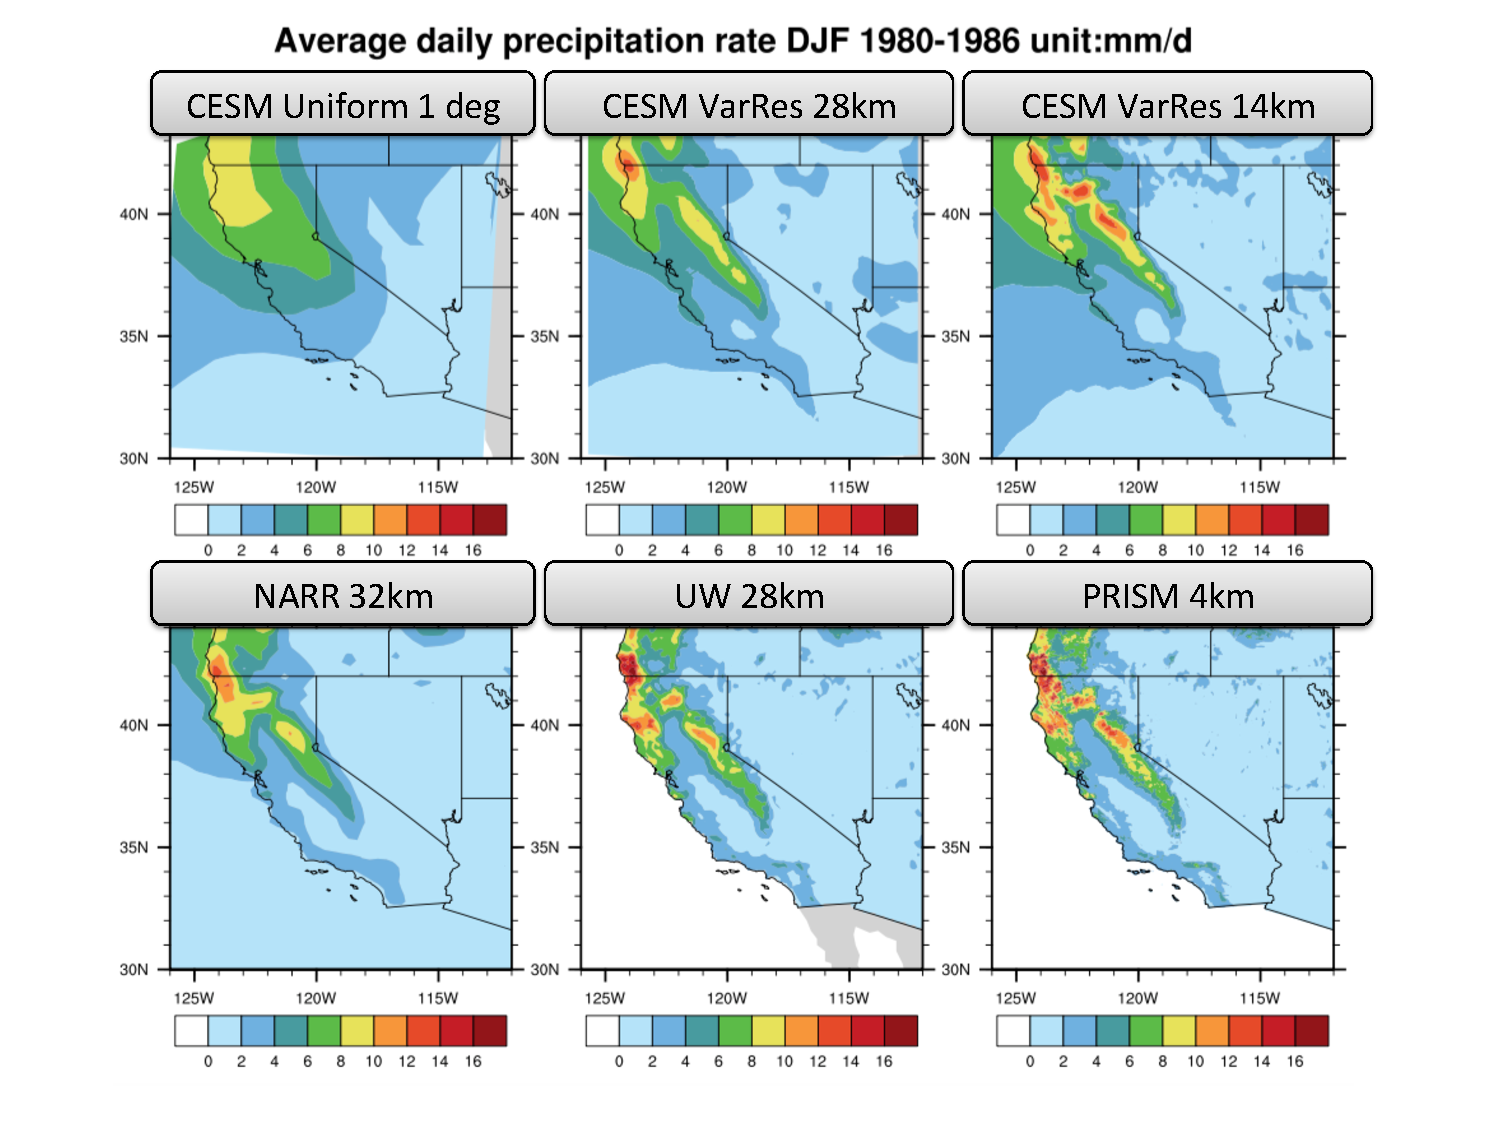
\includegraphics[width=0.8\textwidth]{VariableResolutionPrecipitation.pdf}
\end{center}
\caption{Average daily DJF precipitation over California from (Top Row) three variable resolution model runs at 1 degree (110km), 28 km and 14km over a 7-year period and (Bottom Row) NARR (reanalysis), UW (gridded) and PRISM (gridded) datasets over the same period.} \label{fig:VarResPrecipitation}
\end{figure}

As shown by the most recent snow model intercomparison project (SnowMIP2), a comprehensive assessment of 33 snow models with varying complexity and intended development purpose, no model was shown to perform best across a range of discrete locations in the Northern Hemisphere \citep{rutter2009SnowMIP2}.  Further complications arose in the intercomparison project when canopy interactions were assessed as models performed differently with vegetated and non-vegetated environments.  \citet{rutter2009SnowMIP2} found that a key indicator of more optimal performance in a snow model is its ability to characterize vegetation cover, winter temperature characterization, and performance across a multitude of variables (e.g. snow cover, snow depth, and snow water equivalent).
    
CLM (version 4.0) utilizes a grid cell by grid cell specification routine that breaks each model cell into a unique combination of land unit types including: glacier, lake, urban, vegetated, and wetland \citep{lawrence2011parameterization}.  The vegetated component of the grid cell is further broken down into various soil types which are then characterized by 15 unique, plus non-vegetated, Plant Functional Types (PFTs) \citep{lawrence2011parameterization}. CLM4 PFTs include: five evergreen species and six deciduous species for temperature, boreal, and tropical climates, three grasses for arctic and non-arctic climates (with C-3 and C-4 variations) and a few staple cereal crops \citep{lawrence2011parameterization}.  PFT cover is derived from the Moderate Resolution Imaging Spectroradiometer (MODIS) satellite data at 0.5$^{o}$ resolution with canopy heights for each of the PFTs assumed to be constant and canopy diameters ranging from 0.5 meters (crops, grasses, and shrubs) to 35 meters (trees) \citep{lawrence2011parameterization}.  

As discussed previously, PFT types and percent cover of PFTs within each vegetated land-unit play a crucial role in shaping snowpack trends. This is because the interaction between the canopy and snowpack are PFT specific for biogeochemical, radiative, and hydrological processes including: interception, throughfall, canopy drip, water removal via transpiration, and optical property interactions based on leaf angle and specific PFT \citep{lawrence2011parameterization}.  Therefore, CLM4 provides a relatively complex representation of snowpack and its biogeophysical interactions within a GCM framework, lending itself well to this study.   A higher resolution dataset for PFT type would have been beneficial for this study, to capitalize on the higher resolution (less than 0.5$^\circ$) VRGCM grids implemented into both CAM5 and CLM4, however none were found.

\begin{wrapfigure}{r}{2.5in}
\centering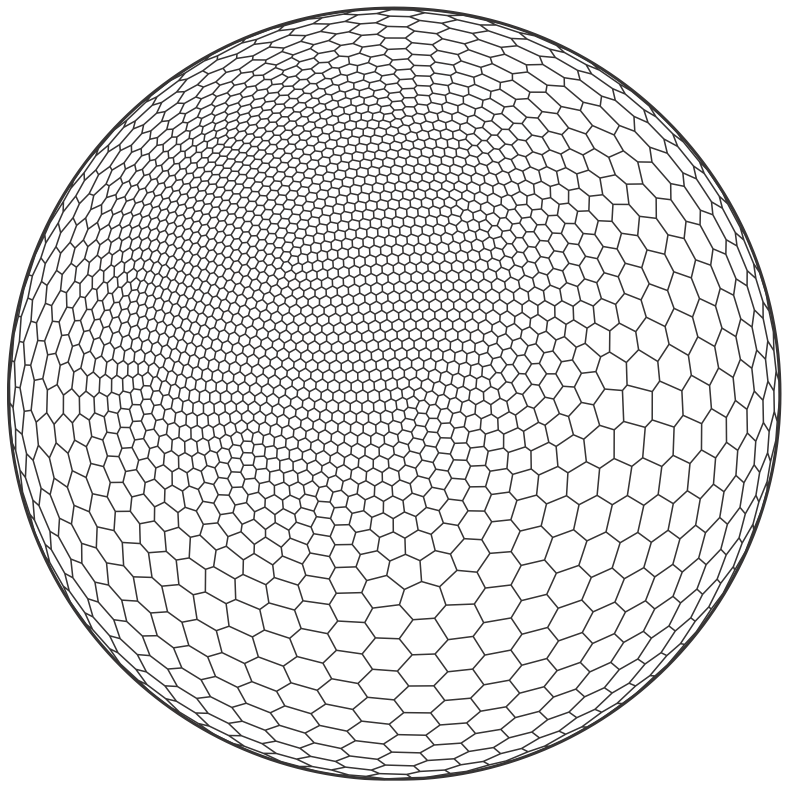
\includegraphics[width=2.2in]{RinglerGrid.png}
\caption{A conformal icosahedral-Voronoi stretched grid used in the MPAS model.} \label{fig:MPAS-AdaptedGrid}
\end{wrapfigure}

The parameterizations of snowpack within CESM are based primarily on work done by \citet{anderson1976point}, \citet{jordan1991one}, and \citet{yongjiu1997land}. These parameterizations characterize several important state variables for snowpack including: the mass of water, mass of ice, snowpack layer thickness, temperature profile of the snowpack layer, black carbon and mineral deposition, and snowpack aging and optical properties \citep{lawrence2011parameterization}. Through the characterization of these state variables, in numerically discretized equations, a five layer snow model with dynamic compaction, water transfer, and energy transfer was created \citep{lawrence2011parameterization}, the SNow and Ice Aerosol Radiation (SNICAR) model.  The SNICAR model replaced the CLM3 snow model which was used in the SnowMIP2 intercomparison project.  This has resulted in a much more complete representation of snowpack, and its tendencies, than its predecessor used in SnowMIP2.

The MPAS model \citep{WCSJBKMGDLDFSHPTDR2012MWR} is a recently developed multi-resolution dynamical core and ocean model which uses a centroidal Voronoi mesh consisting of hexagons and pentagons and a smooth transition between regions of coarse and fine resolution.  The Voronoi mesh has the advantage of maximizing uniformity of elements across the globe and preserving scalability on massively parallel machines.  Further, this model has been developed using a novel approach \citep{JTTDRWCSJBK2009JCP} which is effective at maintaining geostrophic balance and preserves the desirable properties of atmospheric waves.  This model has the additional advantage of being built upon the substantial experience that went into the development of the WRF model.  A depiction of the smoothly varying grid used by the MPAS model is shown in Figure \ref{fig:MPAS-AdaptedGrid}.

\subsection{Research Tasks}

This proposal incorporates both a computational and a scientific focus. The computational focus will utilize a suite of modeling tools to improve model resolution over California, and provide an evaluation on the effectiveness of these tools for capturing small-scale features. Studies of enhanced resolution via dynamical downscaling (using the WRF regional model) and variable resolution modeling using the fully integrated VRGCM in CESM will be performed. The scientific focus will use the simulation data to determine whether the dynamically downscaled model and VRGCMs are able to capture the 20th century trend in snowpack loss and and isolate model predictions on the future behavior of these snowpack fields.

The tasks required for this project will be completed in three stages: In the first stage, control simulations will be run over the 1980-2005 time period. Snowpack indicators will then be compared against the bevy of observational products highlighted above to verify consistency between the modeled climatology and observations. In the second stage, the VRGCMs will be used to execute a similar set of simulations over a similar temporal period and the results compared against the control simulation to determine any inherent differences in the behavior or predictive capability of the VRGCMs versus the dynamically downscaled WRF simulation. In the third stage, the VRGCM simulations will be extended to a predictive ensemble over the 2025-2050 time period using both Climate Variability and Predictability (CLIVAR)-type Atmospheric Model Intercomparison Project (AMIP) forcings (prescribed sea-surface temperatures) and fully coupled global atmospheric simulations with a fully coupled ocean. Results from the predictive simulations will be compared to the control simulations to determine the mean behavior and variability of the snowpack under future warming scenarios.

The study regions are identified in Figure \ref{}.

{\color{red} Map of west coast study regions?}

\subsubsection{(T1) WRF simulations (1980-2005)}

An ensemble of control simulations will be constructed using the limited area two-way WRF model run over the US west coast at high resolution (10km resolution at the highest refinement level, with additional nested refinement levels at 20km and 55km). The outer domain will approximately cover 15N to 60N and 150W to 100W. Initially an ensemble of 10 perturbed initial condition runs will be used, with additional simulations added as needed. ERA reanalysis data will be used for the initial conditions, lateral boundary conditions and prescribed sea-surface temperatures. The period of integration will be 1980-2005 with the WRF simulation nudged to the reanalysis data to reduce disagreement between ERA and WRF. Snow products such as snow depth, snow water equivalent, and snow cover will obtained from the output data.  These model outputs will then be compared over the simulation period with all of the observational datasets highlighted above, so as to quantify the quality of the coupled regional-global model results. Precipitation results, which can be very sensitive to model and topographical resolution, will also be compared with rain gauge data to verify consistency with historical observations.  Additionally, surface energy budgets and temperature profiles will be assessed to identify behavioral traits in snowpack tendencies.

Once the model output is obtained, correlations between observational products and model outputs will be computed and compared at both the regional and grid point scale to determine any intrinsic biases in the simulation results. Specifically, these biases may be due to particular sensitivities in the model, such as issues due to unresolved topographical forcing or in the physical treatment of precipitation. The use of an ensemble of simulations is particularly useful for determining the statistics of the climatology generated in each case, including the mean and variance associated with each of the variables of interest.

\subsubsection{(T1) VRGCM assessment simulations (1980-2005) and tuning}

An analogous approach to section 1.4.1 will now be applied  for  the  CESM  (CAM-SE and CLM4.0) and MPAS using built-in support for variable resolutions.  Specifically, these models will be run with a 100km base resolution refined to 14km and 28km regional resolution. For the CESM model a multi-level refined grid, shown in Figure \ref{fig:CESMVarResMeshes}, will be used with three levels of refinement from a background 110km (1$^{o}$) resolution. The region of high resolution will be chosen to closely correspond to the region of refinement for the WRF model.  Sensitivity of the model to topographic smoothing and choice of convective scheme will be assessed.  %One experiment will also examine whether simulation results can be improved by nudging towards the reanalysis data over the duration of the integration.

Again the assessment period will be 1980-2005, and both models will be driven using global prescribed SSTs (in correspondence with the AMIP protocol).  At least three ensemble members will be used for this assessment. Model results will be compared over the 1980-2005 time frame with snowpack observational products. Further, results from the VRGCMs will be compared against the ensemble WRF simulations. This procedure will again allow quantification of biases associated with the VRGCMs and if any additional tuning is required to produce more realistic simulation results.  Specifically, topographical smoothness has been identified as one substantial source of uncertainty in these simulations, especially for the purposes of computing statistics related to snowpack Figure \ref{f3}.

\subsubsection{(T1) Analysis of 1980-2005 simulations}

Using the ensemble of model simulations, snowpack information (seasonally averaged SWE, snow depth, snow cover, interannual variability, spatial distribution) will be assessed for all relevant summary statistics (e.g. mean, variance, quartile ranges, summed totals, etc.). Both large-scale (west coast) and local assessments (within individual study regions) will be performed, with particular interest in determining trends in the spatial distribution and summary statistics of snowpack over this period.

%Further, the spatial dependence of these quantities will be used to provide local assessments in each of the study regions.

\subsubsection{(T2) Analysis of the Community Land Model}

SNOTEL stations are perhaps the most reliable resource for mountain snowpack measurements, but their distribution and altitude is not representative of the element-averaged values provided by model simulations.  Nonetheless, as a column model, CLM is theoretically capable of assessing snowpack at pointwise locations when driven by model meteorology.  Consequently, towards the goal of evaluating the capability of the model to match observational data, this proposal will assess the ability of CLM to match SNOTEL measurements over the validation period (1980-2005) when driven by both observed meteorology and interpolated meteorology from variable resolution simulations.  Mean snow depth and SWE will be assessed.  {\color{red} More here from Mark Flanner?}

\subsubsection{(T3) VRGCM Predictive Simulations (2040-2060 and 2080-2100)}

Once the VRGCMs have been assessed over the 1980-2005 time period, the next step is the use of this model for prediction of future snowpack.  Future assessment will be performed over two 20 year periods representing mid-century (2040-2060) and late century (2080-2100) climatology.  At least three ensemble members will be used for each period.  Sea-surface temperatures and greenhouse gas concentrations for the simulation periods will be derived from CMIP5 fields based on the Intergovernmental Panel on Climate Change (IPCC) fifth assessment report Representative Concentration Pathways (RCP) 8.5 and 4.5.

The analysis will be analogous to the model validation tasks (T1), although in this task differences between future snowpack and present snowpack will be identified.  This task will focus on both total west coast SWE, as well as total SWE in each of the study regions.

%To limit the computational cost of the predictive model and allow for additional experiments, only the 2025-2050 simulation period will be considered initially. 

%A suite of experiments will be pursued, as listed in Table 1 using climate forcings derived from the Intergovernmental Panel on Climate Change (IPCC) fifth assessment report Representative Concentration Pathways (RCP), as well as present day control simulations and CLIVAR-type 2xCO2 experiments. Sea-surface temperatures will either use present day values following the AMIP framework, modified sea surface temperatures (+2 degrees warmer) or will be obtained online via a fully coupled ocean model.

%\begin{table}[t1]
%\begin{center}
%\caption{Predictive experiments for the VRGCM simulation over the 2025-2050 simulation period}
%\vspace{0.3cm}
%\begin{tabular}{|l|r|r|} \hline
%Experiment & Climate Forcing & Sea-Surface \\\hline
%Control & Present day & Present day (AMIP) \\
%2xCO2 & 2xCO2 & Present day (AMIP) \\
%SST+2 & Present Day & SST+2 (AMIP) \\
%2xCO2, SST+2 & 2xCO2 & SST+2 (AMIP) \\
%8.5-FULL & RCP8.5 & Fully coupled \\
%2.6-FULL & RCP2.6 & Fully coupled \\\hline
%\end{tabular}
%\end{center}
%\end{table}

\subsubsection{(T4) Detection and Characterization of Atmospheric Rivers}

Atmospheric rivers (ARs) are meteorological phenomena characterized by long, narrow plumes of increased atmospheric moisture stretching between the subtropics and the midlatitudes regions.  These features are responsible for 30\%-50\% of total US west coast precipitation, particularly during winter months, and 30\%-40\% of total seasonal SWE \citep{dettinger2011atmospheric}.  The majority of total seasonal SWE contribution from ARs will often occur as a result of 1-2 extreme AR events \citep{guan2010extreme}.  ARs are usually between 400 to 600\ km wide, and so at global model resolutions of $1^\circ$ are mostly unresolved, occupying as few as four grid cells in the latitudinal direction.  The variable resolution simulations performed under research tasks (T1) and (T3) will be invaluable to the study of these features: Not only will atmospheric rivers be much better resolved at 28km and 14km resolution, but the variable resolution grids used in this study (see Figure \ref{fig:CESMVarResMeshes}) have been designed to represent a swath of the eastern Pacific that is most relevant for the study of these features.  Specifically, this proposal will utilize the higher model resolution achieved in the variable resolution framework to determine how ARs will respond to changes in circulation and how major snowfall events associated with ARs will change under future climate.

This proposal will use automated atmospheric river detection and characterization for understanding AR events in the variable resolution data \citep{ralph2004satellite, lavers2012detection}.  The characterization of atmospheric rivers will be based on \cite{neiman2008meteorological} and \cite{guan2010extreme}, who use column-integrated water vapor to identify filamentary structures over the eastern Pacific.  The capability to detect these structures will utilize technology from the TempestExtremes software package, a new suite of flexible detection and characterization algorithms developed by the PI for processing large climate datasets.  AR structures will be agglomerated in space using a graph traversal algorithm, and then connected in time by determining overlaps in detections at adjacent time points.  Discrete AR events will then be characterized in terms of point of landfall and total associated precipitation (rainfall and snowfall).  Statistics will then be computed on these quantities including proportion of precipitation associated with AR events, frequency of AR events and mean spatial point of landfall.  This information will then be used for addressing both sensitivity of AR events to grid resolution (using 110km, 28km and 14km datasets) and changes to AR events under future climatology.

%Time series of the frequency, magnitude and other characteristics of extreme weather events over the past century are not well-measured.

%The capability to address the characteristics of atmospheric rivers will rely on the TempestExtremes software package, a new suite of flexible detection and characterization algorithms developed by the PI for processing large climate datasets. This package uses an algorithmic framework known as ``MapReduce'' to first detect candidate events at individual times using specified criteria. Stitching is then used to assess the evolution of related detections over time. The result is an objective calculation of the climate indicator that can be automated and parallelized for multiple datasets.  For atmospheric rivers, algorithmic detection is usually performed via {\color{red} [Methodology?]}

\subsubsection{(T5) Reporting}

{\color{red} [US Climate assessment?]}

\subsubsection{Plan of Work}

PI Ullrich will be the primary administrator for the project, and will be responsible for managerial and administrative decisions, including planning, scheduling and oversight of research tasks, plus reporting of technical progress. He will be the primary contact on this project and will be the point of engagement for project collaborators and their teams. He will further be responsible for ensuring that sufficient computational resources are available for continued progress on the project. The majority of the requested funds will be used to pay for one full-time Graduate Student Researcher (GSR) who will pursue this research as part of their Ph.D. research. The GSR will be advised full-time by the PI at UC Davis. In addition, funding will be used to reimburse the PI for one month of salary, which will be used to fund a eight percent commitment of effort to support the GSR on this work. The PI and GSR will meet once per week to discuss the progress and status of the project. Milestones for this project are given below:

\begin{tabularx}{\textwidth}{cX}
\hline
\textbf{Year 1} & $\cdot$ Intercomparison of metrics for snowpack \\
& $\cdot$ WRF, CESM and MPAS validation period ensemble simulations \\
& $\cdot$ Analysis of validation period ensemble simulations \\
\hline
\textbf{Year 2} & $\cdot$ Analysis of reproducibility of SNOTEL results from CLM \\
& $\cdot$ CESM and MPAS future simulations (RCP) \\
& $\cdot$ Initial analysis of future simulations (RCP) \\
\hline
\textbf{Year 3} & $\cdot$ Detection and characterization of atmospheric rivers \\
& $\cdot$ Final analysis and report of project conclusions \\
\hline
\end{tabularx}

We expect results and research progress will be presented at regular scientific meetings, including meetings of the American Geophysical Union (AGU) and the American Meteorological Society (AMS). This work will also be presented at the CESM annual working group meeting and CESM atmospheric working group meeting. We further anticipate that we will publish at least one peer-reviewed article in each year.

\subsubsection{Prior NSF Support}

\end{document}